\section{Motivation}
Lucene is a widely used text search engine library that relies on managed runtimes for indexing and querying large datasets efficiently. TeraHeap, a state-of-the-art memory system, extends the managed heap beyond DRAM by partitioning it into a primary heap (H1) in DRAM and a secondary heap (H2) mapped to a slower memory tier such as NVMe SSD. This design reduces garbage collection (GC) overhead by limiting GC operations to H1, while H2 provides additional capacity for less frequently accessed data.

However, TeraHeap statically divides DRAM between H1 and the page cache for H2 at JVM launch time, which introduces significant limitations. If H1 is too small, Lucene experiences high GC overhead due to frequent collections, impacting query and indexing latency. Conversely, if the DRAM page cache for H2 is too small, accessing index segments stored in H2 incurs high I/O latency, degrading search performance. Because Lucene workloads exhibit varying memory demands, such as bulk indexing phases which require large heaps, while read-heavy query phases benefit from a larger page cache. Moreover, a static DRAM division is not able adapt to these changes, leading to suboptimal performance.

These limitations motivate our approach: dynamically resizing the primary heap (H1) at runtime in TeraHeap to better match Lucene’s changing memory needs. By adjusting H1 size based on GC and I/O costs, we enable Lucene to maintain low GC overhead during indexing and benefit from a larger page cache during query processing, ultimately improving overall performance under DRAM constraints.

The figure \ref{fig:graph} illustrates the breakdown of Lucene’s total execution time into GC time and non-GC (other) time under different page cache configurations. The x-axis represents the fraction of DRAM allocated to the page cache (10\%, 20\%, 30\%, 40\%, etc.), while the y-axis shows the average total execution time in seconds for each configuration.

\begin{figure}[htbp]
  \centering
  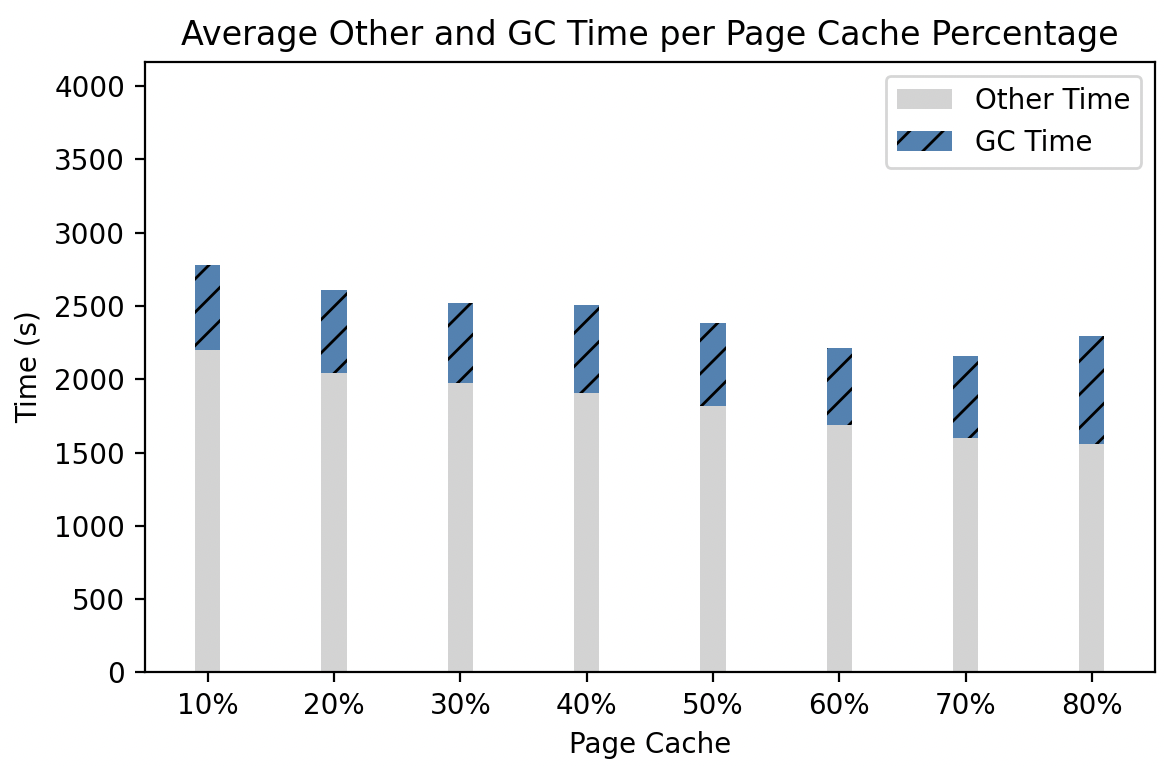
\includegraphics[width=1\columnwidth]{fig/numbers.png}
  \caption{Graph of different H1/page cache partitionings}
  \label{fig:graph}
\end{figure}

At low page cache allocations (10\% to 30\%), the GC time is minimal relative to total execution time. However, as the page cache share grows (40\% to 60\%), GC time steadily increases. This is because increasing page cache size reduces the available DRAM allocated to H1, resulting in a smaller primary heap. A smaller heap triggers more frequent garbage collections, leading to higher GC overhead.
The grey part of each bar represents the time spent executing Lucene and system operations excluding GC. As the page cache share increases, the non-GC time decreases. This is because a larger page cache reduces I/O latency when accessing index segments stored in H2 (SSD) such as Lucene's query cache.
The graph captures the tradeoff in TeraHeap’s static DRAM partitioning: \vspace{-0.5em} 
\begin{itemize} 
  \item Allocating more DRAM to H1 results in a larger heap, reducing GC time but yielding a smaller page cache, which increases I/O latency and non-GC execution time.
  \item Allocating more DRAM to the page cache reduces I/O latency and non-GC execution time but increases GC overhead due to the smaller H1.
\end{itemize} 
\vspace{-0.5em}
The graph indicates that there is potential for optimization by introducing a dynamic heap resizer that adjusts the H1 size at runtime based on workload phases and memory pressure. Such an approach could balance the trade-offs between configurations by reducing GC time during indexing while also minimizing I/O latency during query processing. 

